\documentclass{beamer}

\usepackage[utf8]{inputenc}
\usepackage{csquotes}
\usepackage{latexsym,amsmath,xcolor,multicol,booktabs,calligra, animate, subfig}
\usepackage{graphicx,pstricks,listings,stackengine, bbm}
\usepackage{tikz}
\usetikzlibrary{fit,tikzmark}   
\usepackage{booktabs,cellspace}
\usepackage{color, colortbl}
\usepackage{hyperref}
\usepackage{natbib}
\usepackage{color}
\usepackage{changepage} % in your preamble

%Information to be included in the title page:
\title{AERE @ WEAI\\
Rawls for Environmental Justice}
\author{Lauren Beatty\\ \href{mailto:lbeatty@edf.org}{lbeatty@edf.org} \\
\vspace{.3cm}
Matthias Fripp\\
\href{mailto:matthias@energyinnovation.org}{matthias@energyinnovation.org}}
\institute{Environmental Defense Fund}
\date{June 21, 2024}


%% Tikz
\usepackage{tikz}
\usetikzlibrary{shapes.geometric, arrows}

\tikzstyle{start} = [rectangle, rounded corners, 
minimum width=3cm, 
minimum height=1cm,
text centered, 
draw=black, 
fill=orange!30]

\tikzstyle{process} = [rectangle, 
minimum width=3cm, 
minimum height=1cm, 
text centered, 
text width=3cm, 
draw=black, 
fill=blue!30]

\tikzstyle{stop} = [rectangle, rounded corners, 
minimum width=3cm, 
minimum height=1cm,
text centered, 
draw=black, 
fill=green!30]

\tikzstyle{arrow} = [thick,->,>=stealth]


\logo{\includegraphics[height=.5cm]{EDF_color_webRGB_2022 (2).png}\hspace*{.03\paperwidth}\vspace{.01\paperwidth}}


%Color Pallete
\definecolor{EDFblue}{RGB}{0.0, 51, 204}
\definecolor{EDFgreen}{RGB}{0, 153, 51} 
\definecolor{EDFlightgreen}{RGB}{161, 226, 20}
\definecolor{EDFcyan}{RGB}{51,204,255}
\setbeamercolor{structure}{fg=EDFblue} 
\setbeamercolor{button}{bg=EDFblue,fg=white}
\setbeamertemplate{navigation symbols}{}
\newcommand{\nologo}{\setbeamertemplate{logo}{}} % command to set the logo to nothing


\hypersetup{colorlinks,linkcolor=EDFblue,urlcolor=EDFblue}


\begin{document}

\frame{\titlepage}

\section{Introduction}

\begin{frame}{Introduction}
\begin{itemize}
    \item Air pollution is responsible for $\sim 7$ million deaths annually (\href{https://www.who.int/health-topics/air-pollution#tab=tab_2}{WHO}).
    \item In the U.S.,  Black and non-Hispanic white people are exposed to higher levels of air pollution than other groups. Low income people are exposed to higher pollution levels than high income people, controlling for race \citep{Thind2019FineGeography}.
    \item \citet{Lelieveld2015TheScale} estimate that power generation is linked with 31$\%$ of premature mortality caused by outdoor air pollution in the U.S.
\end{itemize}

    \textbf{How can we reduce air quality \textit{equitably?}}
\end{frame}

\begin{frame}{Previous Work}
\begin{itemize}
    \item \citet{Sergi2020OptimizingBenefits} include co-benefits involved with reducing electricity generation from fossil fuels in the objective function.
    \item citep{Goforth2022AirStrategies} and \citep{Shawhan2024PoliciesAmericans} project how the electricity transmission might affect the distributional consequences of air pollution exposure.
\end{itemize}
\end{frame}

\begin{frame}{Our Approach}
    \begin{enumerate}
        \item Use EPA emissions data to calculate emissions rates (Pounds per MWh)
        \item Use InMap Source-Receptor Matrix to calculate how one MWh of generation for each resource affects population-weighted average exposure for different groups.
        \item Use Switch to calculate least-cost planning costs.
        \item Modify and run Switch to minimize air pollution exposure subject to a cost constraint.
    \end{enumerate}

\paragraph{Benefits}
\begin{itemize}
    \item Avoids the use of equity weights while still centering distributional concerns.
    \item Still finds low-cost solutions.
    \item Generalizable framework
\end{itemize}
\end{frame}

\begin{frame}{Least-Cost Electricity Planning Models}
\begin{center}
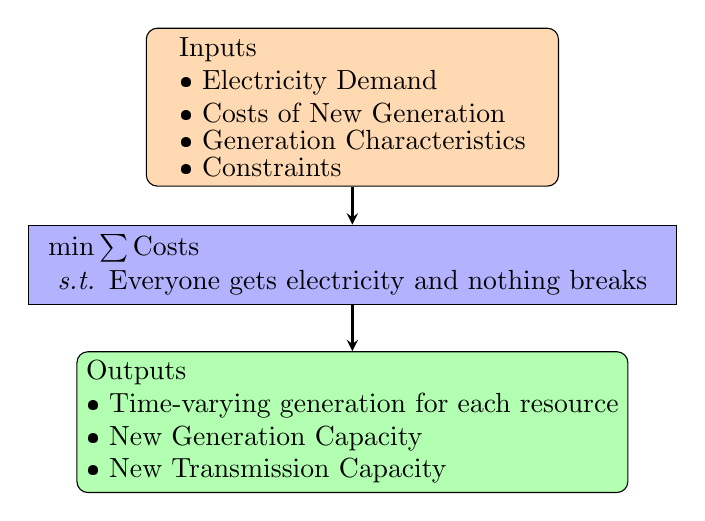
\begin{tikzpicture}[node distance=2cm]
\node (start) [start, text width=5cm] {\shortstack[l]{Inputs\\• Electricity Demand \\ • Costs of New Generation \\ • Generation Characteristics\\
• Constraints}};

\node(obj)[process, below of=start, text width=8cm]{\shortstack[l]{$\min \sum \text{Costs}$ \\ \textit{ 
   s.t.   }\text{Everyone gets electricity and nothing breaks }}};

\node (result) [stop, below of=obj] {\shortstack[l]{Outputs\\• Time-varying generation for each resource \\ • New Generation Capacity \\ • New Transmission Capacity}};

\draw [arrow] (start) -- (obj);
\draw [arrow] (obj) -- (result);

\end{tikzpicture}
\end{center}
\end{frame}

{\nologo
\begin{frame}{Endogenous Exposure}
    \begin{center}
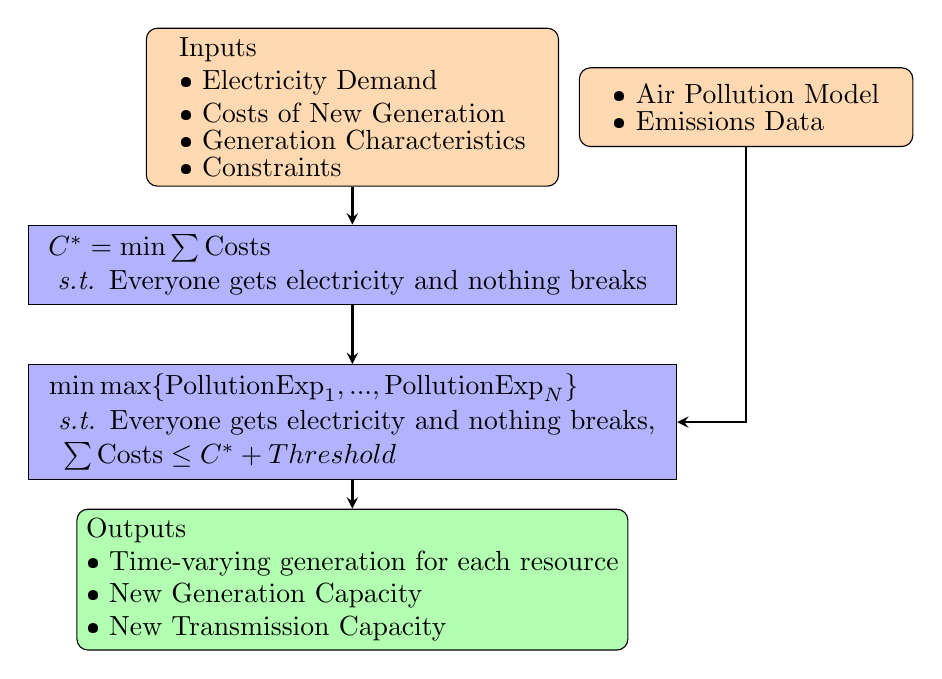
\begin{tikzpicture}[node distance=2cm]

\node (start) [start, text width=5cm] {\shortstack[l]{Inputs\\• Electricity Demand \\ • Costs of New Generation \\ • Generation Characteristics\\
• Constraints}};

\node (air) [start, text width=4cm, right of= start, xshift=3cm] {\shortstack[l]{• Air Pollution Model\\
• Emissions Data}};

\node(obj)[process, below of=start, text width=8cm, xshift=0cm]{\shortstack[l]{$C^* = \min \sum \text{Costs}$ \\ \textit{ 
   s.t.   }\text{Everyone gets electricity and nothing breaks }}};

\node(obj2)[process, below of=obj, text width=8cm, xshift=0cm]{\shortstack[l]{$\min \max\{\text{PollutionExp}_1,...,\text{PollutionExp}_N\}$ \\ \textit{ 
   s.t.   }\text{Everyone gets electricity and nothing breaks,} \\
    $\text{      }\sum \text{Costs} \leq C^*+Threshold$ }};

\node (result) [stop, below of=obj2] {\shortstack[l]{Outputs\\• Time-varying generation for each resource \\ • New Generation Capacity \\ • New Transmission Capacity}};

\draw [arrow] (start) -- (obj);
\draw [arrow] (air) |- (obj2);
\draw [arrow] (obj) -- (obj2);
\draw [arrow] (obj2) -- (result);


\end{tikzpicture}
\end{center}
\end{frame}}


\begin{frame}{A Point About Calculus}
    \includegraphics[width=0.48\textwidth]{Figures/Slide Pictures/Transmission1.png} \includegraphics[width=0.48\textwidth]{Figures/Slide Pictures/Transmission2.png}

    The effect of deviations from the least-cost optimum will depend on the shape of the objective function.  This is an \textit{empirical} question!\\
    \vspace{.5cm}
    $\Rightarrow$ Perhaps you can get large improvements in health at only modest increases in cost.
\end{frame}


\begin{frame}{Data}
    
\end{frame}

\begin{frame}{Results}
    \begin{itemize}
        \item Imperfect correlation between emissions rates, and effects on pollution.
        \item Modest budgets can dramatically reduce air pollution exposure from electricity generation.
        \item Air quality improvements exhibit decreasing marginal returns.
        \item The mechanisms for reducing air pollution are:
        \begin{itemize}
            \item Expanding wind and solar
            \item Decreasing coal generation faster
            \item Changing the spatial distribution of remaining fossil generation
            \item Increases in transmission
        \end{itemize}
    \end{itemize}
\end{frame}

\begin{frame}{Imperfect Correlation Between Emissions Rates and Effects on Pollution}
\includegraphics[width=0.49\textwidth]{Figures/EndogenousPaper/emissions_by_technology.png}
\includegraphics[width=0.49\textwidth]{Figures/EndogenousPaper/exposure_by_technology.png}
\end{frame}

\begin{frame}{Large Improvements in Air Quality at Modest Costs}
    \centering
    \includegraphics[width=0.8\textwidth]{Figures/EndogenousPaper/exposure_by_scenario_2050.png}
\end{frame}

\begin{frame}{Decreasing Marginal Returns}
    \centering
    \includegraphics[width=0.8\textwidth]{Figures/EndogenousPaper/exposure_cost_PPF.png}
\end{frame}


\begin{frame}{Decreasing Fossil and Increasing Renewable Generation}
\begin{adjustwidth}{-3em}{-1.5em}

    \centering
    \begin{minipage}{1.1\textwidth}
        \centering
        \includegraphics[width=0.32\textwidth]{Figures/EndogenousPaper/Dispatch_Relative_by_scenario_2027.png} \hfill
        \includegraphics[width=0.32\textwidth]{Figures/EndogenousPaper/Dispatch_Relative_by_scenario_2030.png} \hfill
        \includegraphics[width=0.32\textwidth]{Figures/EndogenousPaper/Dispatch_Relative_by_scenario_2035.png}
    \end{minipage}
    
    \vspace{0.5cm}
    
    \begin{minipage}{1.1\textwidth}
        \centering
        \includegraphics[width=0.32\textwidth]{Figures/EndogenousPaper/Dispatch_Relative_by_scenario_2040.png} \hfill
        \includegraphics[width=0.32\textwidth]{Figures/EndogenousPaper/Dispatch_Relative_by_scenario_2045.png} \hfill
        \includegraphics[width=0.32\textwidth]{Figures/EndogenousPaper/Dispatch_Relative_by_scenario_2050.png}
    \end{minipage}
\end{adjustwidth}
\includegraphics[scale=.3]{Figures/EndogenousPaper/Legend_2050.png}
\end{frame}


\begin{frame}{Increasing Renewable Generation}
    \centering
    \includegraphics[width=0.8\textwidth]{Figures/EndogenousPaper/solar_generation_map.png}
\end{frame}


\begin{frame}{Increasing Renewable Generation}
    \centering
    \includegraphics[width=0.8\textwidth]{Figures/EndogenousPaper/wind_generation_map.png}
\end{frame}

\begin{frame}{Decreasing Coal Faster}
    \centering
    \includegraphics[width=0.8\textwidth]{Figures/EndogenousPaper/coal_generation_map_2027_200B.png}
\end{frame}

\begin{frame}{Changing the Spatial Distribution of Remaining Fossil Generation}
\centering
\includegraphics[width=0.8\textwidth]{Figures/EndogenousPaper/naturalgas_generation_map.png}
\end{frame}
\begin{frame}{Transmission/Capacity Substitution}
    \centering
    \includegraphics[width=\textwidth]{Figures/EndogenousPaper/transmission_capacity_substitution.png}
\end{frame}

\begin{frame}{Thanks!}
\label{Thanks}


    Please feel free to contact me at:
    \href{mailto:lbeatty@edf.org}{lbeatty@edf.org}\\
    \vspace{1cm}
\end{frame}

\begin{frame}{References}
\newpage
\bibliographystyle{jpe}
%\bibliographystyle{econometrica}
\bibliography{references.bib}
\end{frame}
\end{document}